\paragraph{\textbf{General framework of unsupervised ML}}

Different from supervised ML, given a dataset $\{\bm{x}_i\}_{i=1}^{M}$ that may or may not have the corresponding labels $\{y_i\}_{i=1}^{M}$, which is generated from some underlying probability distribution $p(\bm{x})$, the application of unsupervised ML is aimed at learning the underlying structure of the data, which may be used for enhancing our understanding on the data, or facilitating the development of training protocols for the supervised ML models. 

It should be emphasised here that the \emph{structure} of the data to be discovered with the unsupervised ML approach is strongly coupled with the specific ML algorithm being used. For examples, signal decomposition analysis [\cref{appendix:signal_decomposition_analysis}] is designed to reveal the global trends across the data by revealing the dominant directions along which the data shows the most pronounced variations. In contrary, multidimensional scaling (MDS) [\cref{appendix:mds}] is designed to preserve the local relationships among the data, which facilitates the discovery of highly similar data points that maybe clustered together, which is the main idea behind clustering analysis [\cref{appendix:clustering_analysis}] that helps to discover recurrent patterns in the data. 

From the probabilistic perspective, the dimensionality reduction analysis (including both the signal decomposition analysis and the MDS) can be viewed as a process that maps the original data $\{\bm{x}_i\}$ to a lower-dimensional latent representation $\{\bm{z}_i\}$, where $\bm{z}_i \in \mathbb{R}^d$ ($d<M$), such that the density of the data being reconstructed in the latent space follows the same distribution as the original data, \emph{i.e.}, $\argmin_{\boldsymbol{\theta}}\mathcal{D}_{\mathrm{KL}}(p_{\boldsymbol{\theta}}(\bm{z})||p(\bm{x}))$. On the other hand, density estimates [\cref{appendix:density_estimation}] tries to develop an ML model (via $\argmin_{\boldsymbol{\theta}}[-\log (p(\bm{x}))]$) that provides the best estimation of the data density in the original space. 

Despite the conceptual simplicity of the unsupervised ML framework, one should be aware of the potential pitfalls when applying unsupervised ML algorithms to analyse the data. One of the most important pitfalls for dimensionality reduction is that it may cause distortion in reflecting the true spatial relationships among the data when projecting the data from a high-dimensional space to a low-dimensional space. Using Principal Component Analysis (PCA) [\cref{appendix:pca}] as an example [see also \cref{fig:PCA_ISOMAP_compare} for an illustration], when analysing a set of data $\{\bm{x}_i\}$ ($\bm{x}_i \in \mathbb{R}^D$), it gives a set of eigenvalues $[\lambda_1,\lambda_2,\cdots,\lambda_D]\in \mathbb{R}^D$. Generally, we have $\lambda_i>0$ $\forall i$, meaning the data has non-zero variance along all $D$ orthogonal directions. However, when projecting all data onto a $d$-dimensional subspace ($d<D$), the data variations along all other $D-d$ directions were ignored, thus such information is lost. In another word, while the peojection along the first $d$ eigenvectors can capture important global trends across the whole dataset, it is not possible to avoid the situations in which some pairs of data $(\bm{x}_m,\bm{x}_n)$ may show more pronouced variations along the $k$-th eigenvector $\bm{v}_k$ ($k>d$), such that the PCA projection may falsely projecting $\bm{x}_m$ and $\bm{x}_n$ very close to each other in the $d$-dimensional subspace, while they are actually far apart in the original $D$-dimensional space. A possible remedy to this problem is to combine dimensionality reduction with clustering analysis [\cref{appendix:clustering_analysis}] that works in the original high-dimensional space,\cite{musil2018machine} which can help to identify the data points that are similar to each other but being wrongly projected to be far apart in the low-dimensional space, or \emph{vice versa}. 

\paragraph{\textbf{Unsupervised ML for atomistic materials and molecular modelling}}

Here, we shall provide a brief account on some of the prominent application of unsupervised ML methods in the field of atomistic materials and molecular modelling. Unlike the previous section on the supervised ML, where we categorised the applications based on the specific target properties to be predicted with the models, here we categorised based on the specific ML algorithms being used. A recent comprehensive review on the applications of unsupervised ML in the field of atomistic materials and molecular modelling can be found in Ref. \citenum{glielmo2021unsupervised}.

\textbf{\textit{Density Estimation}} Estimating the density (or the probability of occurrence) of the data $\rho(\bm{x})$ that is generated from the simulation has important thermodynamic implications in materials modelling, as it is directly related to the free energy of the system via the relationship $F=-k_{\mathrm{B}}T\log \rho(\bm{x})$. For example, the vibrational free energy of solids can be derived from the density of the phonon frequencies $\rho(\omega)$, and similarly, the electronic free energy can be derived from the density of the electronic states $\rho(\epsilon)$. 

One of the most interesting and critical structural motifs in molecular systems is the hydrogen bonds. However, in realistic molecular systems, such as solvents and biomolecules, the atomic environments in which the hydrogen bonds may form are highly dynamic and heterogeneous, making it difficult to adopt a rigid and universal definition of hydrogen banding patterns in these systems. To address this problem, \citet{gasparotto2014recognizing} proposed a fully data-driven agnostic approach to identify hydrogen bonds and other interesting motifs\cite{gasparotto2018recognizing} directly from the simulation data. Here, the underlying probability density of the hydrogen bonding motifs $\rho(\bm{x})$ is first estimated with the kernel density estimation (KDE) method [\cref{appendix:non_parametric_density_estimation}]. Then a Gaussian mixture model (GMM) [\cref{appendix:non_parametric_density_estimation}] is used to fit $\rho(\bm{x})$ thus decomposing $\rho(\bm{x})$ into a set of $k$ Gaussian components, where the optimum number of the Gaussian components $k$ provides a fully data-driven definition of the hydrogen bonding motifs, which also allows one to directly infer the free energy associated with the formation of each type of the hydrogen bonding motifs.

To further illustrate the linkage between density estimation and PES sampling, \citet{rodriguez2018computing} proposed a novel approach to estimate the free energies of biomolecules without the explicit usage of the collective variables, in which the $k$-nearest neighbour (KNN) method is used to estimate the density of the biomolecular conformations $\rho(\bm{x_i})$ in the original high-dimensional space at each sampled point $\bm{x}_i$, from which the corresponding free energy is computed as  $F(\bm{x}_i)=-k_{\mathrm{B}}T\log \rho(\bm{x_i})$. \citet{westerlund2019inflecs} put forward an approach to identify and distinguish the stable and metastable states of biomolecules from the MD trajectory, whereby the desntiy estimation is applied directly to the MD data to determine $\rho(\bm{x})$, from which the gradients and Hessians can be directly computed on $\rho(\bm{x})$ to provide an indication on whether $\bm{x}_i$ corresponds to an energy minimum (stable state) or a saddle point (metastable state). \citet{invernizzi2020rethinking} provided an alternative formulation of metadynamics [\cref{section:metaD}]. Instead of the conventional formulation of metadynamics, where the bias potentials are being added continuously on the collective variables as the simulation progresses, here it viewed the sampling process as one the continuously performs unbiased probability density estimation as a function of the collective variables, until the reweighed free energy from the estimated density converges. Finally, although the density estimate approach was not directly applied, similar concept is adopted to infer the free energy landscape for Li-ion diffusions in solid electrolytes,\cite{gustafsson2023predicting} based on the likelihood of the spatial distribution of the Li-ion positions from statistical sampling. 

Before concluding this part, we would like to point out that, estimating the underlying probability distribution  function $p(\bm{x})$ from the simulation data with density estimate also  (in principle) establishes a critical bridge that allows us to directly draw new samples $\bm{x}^\prime$ from $p(\bm{x})$ with  some targeted probability of occurrences (\textit{e.g.} energy or some other physical properties). This is particularly the case when $p(\bm{x})$ can be described by some basic distributions that are easy to sample from [\cref{tab:discrete_prob_distributions} and \cref{tab:continuous_prob_distributions}]. However, in most realistic situations, the probability distribution $p(\bm{x})$ is high-dimensional, and a many-to-one mapping such that directly inverting $p$ may not be able to lead to a physically feasible new sample $\bm{x}^\prime$. This is where generative modelling become relevant and will be discussed in the later sections.

\begin{figure}[p]
    \centering
    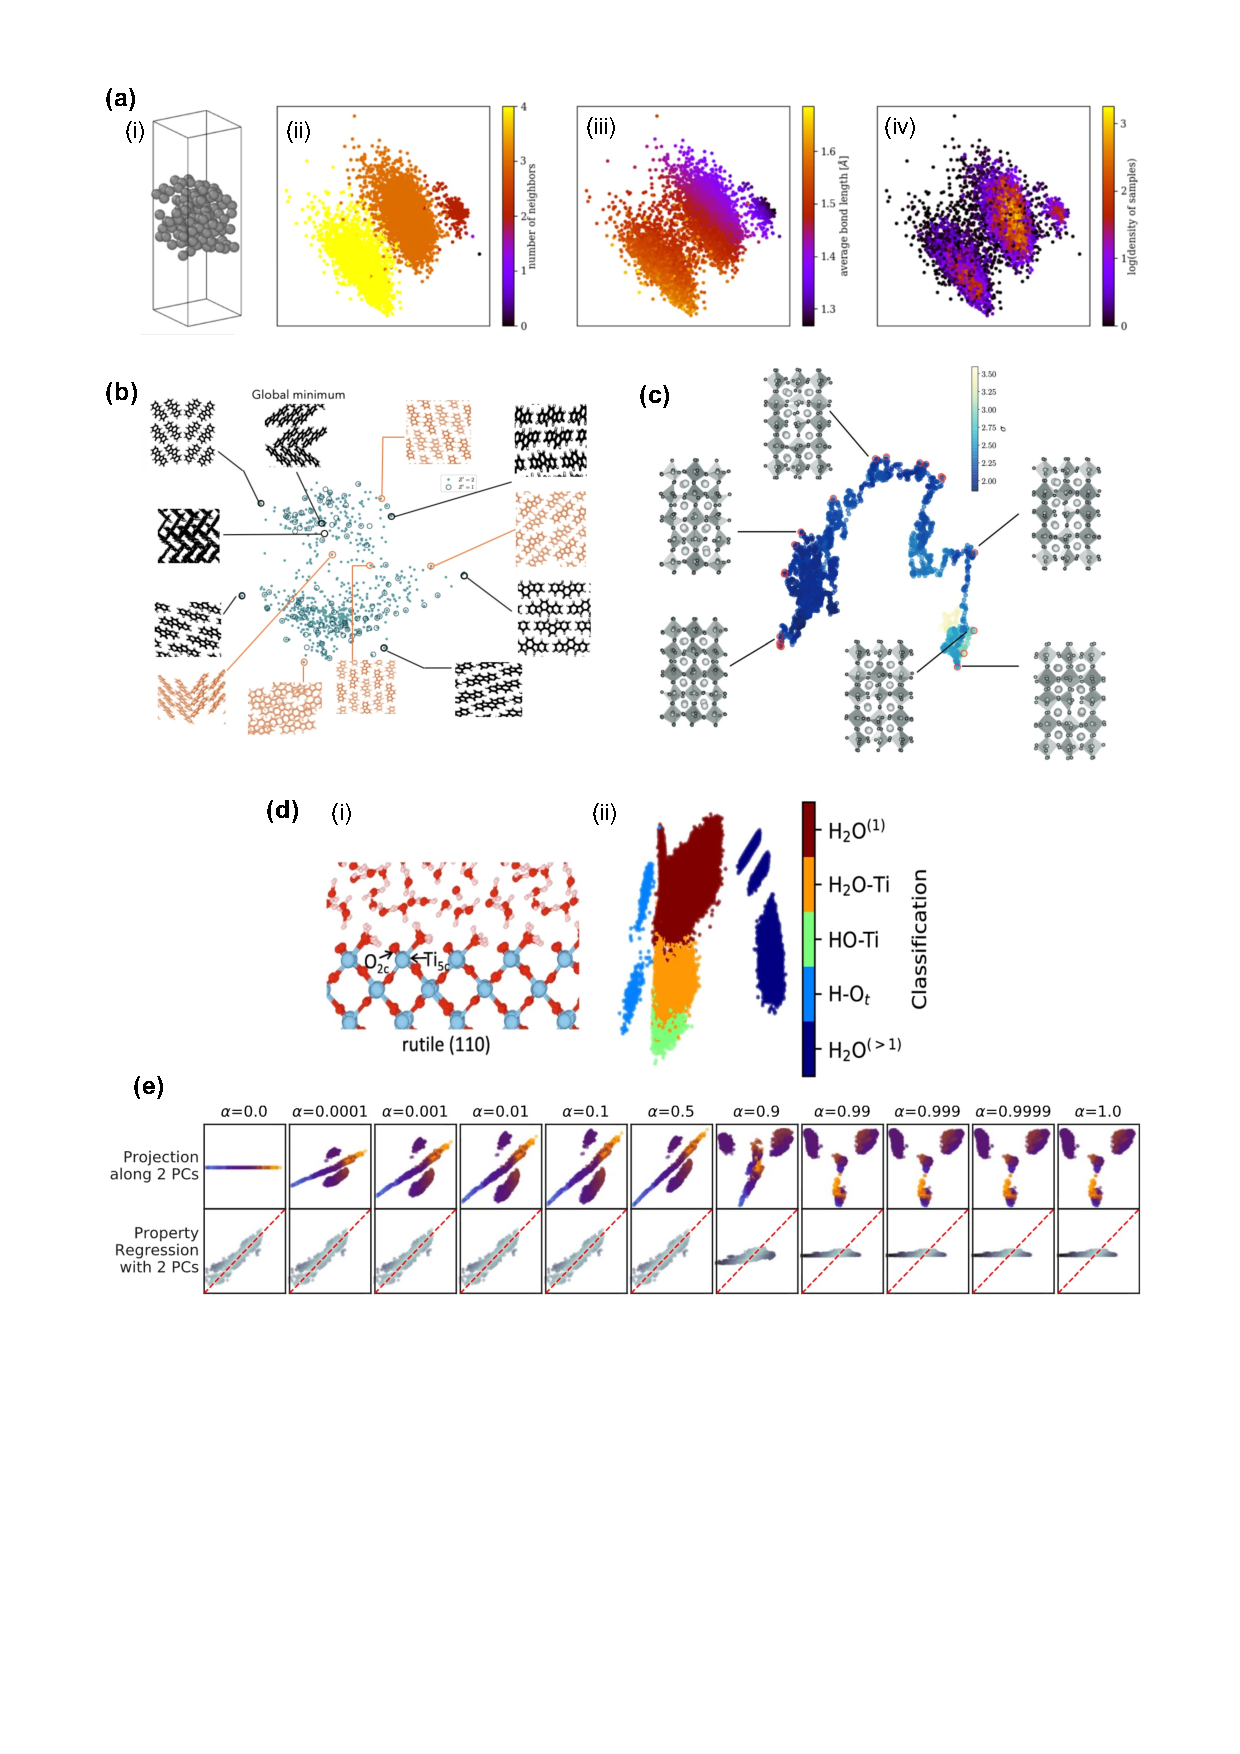
\includegraphics[width=\linewidth]{kpca_examples.pdf}
    \caption{Examples of kernel principal component analysis applied in atomistic molecular and materials modellings. (a) Analysis of the structure-energy landscape of amorphous carbon thin film. (i) A snapshot of the structure\cite{deringer2018computational} (ii-iv) KPCA projection of the atomic environments in amorphous carbon films that are colour coded according to the coordination number, averaged bond length and the he logarithm of the relative probability of each atomic environment.\cite{cheng2020mapping} (b) KPCA map that compares the atomic environments in the predicted crystal structures for an pyrrole azaphenacene in both $Z^\prime=1$ and $Z^\prime=2$ settings.\cite{yang2019interplay}
    (c) KPCA map of the AIMD trajectory for a mixed halide perovskite with each point color-coded according to its vibrational anharmonicity score
    [\cref{eq:anharmonic_score}]. \cite{yang2020mapping}
    All structures in (a-c) are described by the SOAP-based\cite{bartok2013representing,de2016comparing} structural descriptor and similarity kernel. (d) (i) A snapshot of the structure of water on (110) rutile-\ce{TiO2} surface from AIMD and (ii) the corresponding mapping of the hydrogen environments on the same water-oxide interface from KPCA analysis.\cite{zeng2023mechanistic} (e) Principal Covariates Regression (PCovR) performed on the CSD-1000r dataset.\cite{paruzzo2018chemical} Here, a mixing parameter $\alpha$ is applied to toggle between best ridge regression quality (far left) and KPCA (far right) projection for the dataset.\cite{helfrecht2020structure} }
    \label{fig:kpca_examples}
\end{figure}

\textbf{\textit{Kernel Principal Component Analysis (kPCA)}} As a statistical analysis method, PCA has long been used in the field of (bio)molecular simulations to extract the essential dynamics, or equivalently, the dominant collective motions of biomolecules from MD simulations,\cite{amadei1993essential} which was much earlier before ML/AI become popular, particularly for atomistic materials simulations. This is most likely because the usage of bond lengths, angles, and dihedrals makes it trivial to define a set of frame-independent coordinates that capture the essential structural characteristics of molecules, which remains more challenging until the devise of  structural descriptors\cite{musil2021physics} that can equally applied to both materials and molecules. 

Here, we provide a few examples that combine one of the most agnostic structural descriptors, the smooth overlap of atomic positions (SOAP) descriptor\cite{bartok2013representing,de2016comparing} for  mathematically encoding the local chemical environments around each atom,  with the kernel PCA (kPCA) method [\cref{appendix:kpca}] for analysing the structure-property landscapes for molecules and materials, which allows the dominant trends across the whole dataset to be revealed. For examples, amorphous materials are characterised by the lack of long-range order that originates from a large variations in the random local coordination environments around each atom. With the kPCA technique that is applied to the amorphous carbon thin film structures generated from MD simulations,\cite{deringer2018computational} \citet{cheng2020mapping} [\cref{fig:kpca_examples}(a)] demonstrated the variations, diversities and populations of carbon atoms with different numbers of neighbouring atoms (coordination numbers) in amorphous carbon films, which can be applied to facilitate our understanding of how it correlates with the entropic contributions to the free energy of amorphous carbon films. The interplay between molecular structures and hydrogen bonding patterns has a long-lasting interest in the field of organic crystal engineering, and one of the central question is how such an interplay changes the preferences of molecules forming crystals with different numbers of molecules in the asymmetric unit ($Z^\prime$). Our own work on the crystal structure prediction for pyrrole azaphenacene molecules\cite{yang2019interplay} was the first of its kind that revealed the overall high similarity of the local hydrogen bonding environments in the predicted crystal structures for both $Z^\prime=1$ and $Z^\prime=2$ settings [\cref{fig:kpca_examples}(b)]. It also enabled us to propose a global similarity index that aims to quantify the overall similarity between  crystal structure landscapes of two structurally similar molecules. Later, similar techniques were applied to analyse the AIMD trajectories of perovskite photovoltaic materials,\cite{yang2020mapping} providing a visually appealing approach behind the strong correlation between the vibrational anharmonicity  and the changes in the local structural environments of the perovskite materials [\cref{fig:kpca_examples}(c)].

Studying the structures and dynamics of interfacial water on inorganic surfaces with MD has become increasingly popular in the recent years in the field of computational electrocatalysts to deepen our understanding behind the complex physical chemistry on these complex interfaces.\cite{sakong2018electric,kronberg2020revisiting,andrade2020free,kronberg2021reconciling,qin2023cation,chen2023accelerating,yang2023neural} Similar to other (bio)molecular simulations, the challenge here is to reach a quantitative understanding on the diverse structures and dynamics of (un)dissociated water molecules and associated hydrogen bonding patterns in the vicinity of the solid-water interfaces. For this, \citet{zeng2023mechanistic} proposed a set of easy-to-compute descriptors for the proton environments and applied to study the behaviour of water on the low-index \ce{TiO2} surfaces. To overcome the high computational cost associated with projecting a large number of proton environments onto its low-dimensional manifold, a sparsified kPCA method was used, in which a subset of most distinctive proton environments were identified through furtherest-point-sampling (FPS), on which kPCA was applied to compute the first two principal components. Subsequently, the entire dataset can be projected onto these two principal components, leading to a kPCA map that clearly reveals distinguishable clusters, each corresponding to a different type of proton observed in the dataset as shown in \cref{fig:kpca_examples}(d). This is the same as the `landmark' approach that is commonly used in the field of manifold learning, such as in the sketch-map metod,\cite{ceriotti2011simplifying} to reduce the computational cost.

Finally, to enhance the capability of KPCA method in producing meaningful structure-property relationships from atomistic modellings, \citet{helfrecht2020structure} showcased the working principles behind the Principal Covariates Regression (PCovR) approach. Here, the supervised regression and the unsupervised dimensionality reduction are combined together through minimising a loss function $\ell_{\mathrm{PCovR}}=\alpha\ell_{\mathrm{proj}}+(1-\alpha)\ell_{\mathrm{reg}}$, in which a weighting parameter $\alpha$ is applied to toggle between the best projection quality (when $\alpha=1$) and the best regression quality (when $\alpha=0$). With this approach, one can obtain a low-dimensional representation of the data that is not only able to capture the dominant trends across the whole dataset, but also able to reveal the structure-property relationships in the dataset. As shown in \cref{fig:kpca_examples}(e), the PCovR map of the CSD-1000r dataset\cite{paruzzo2018chemical} with $\alpha=0.5$ is able to reveal the overall structural trends across the dataset, whilst showing a clear correlation between the changes in the target properties and the first two principal components.

\begin{figure}[p]
    \centering
    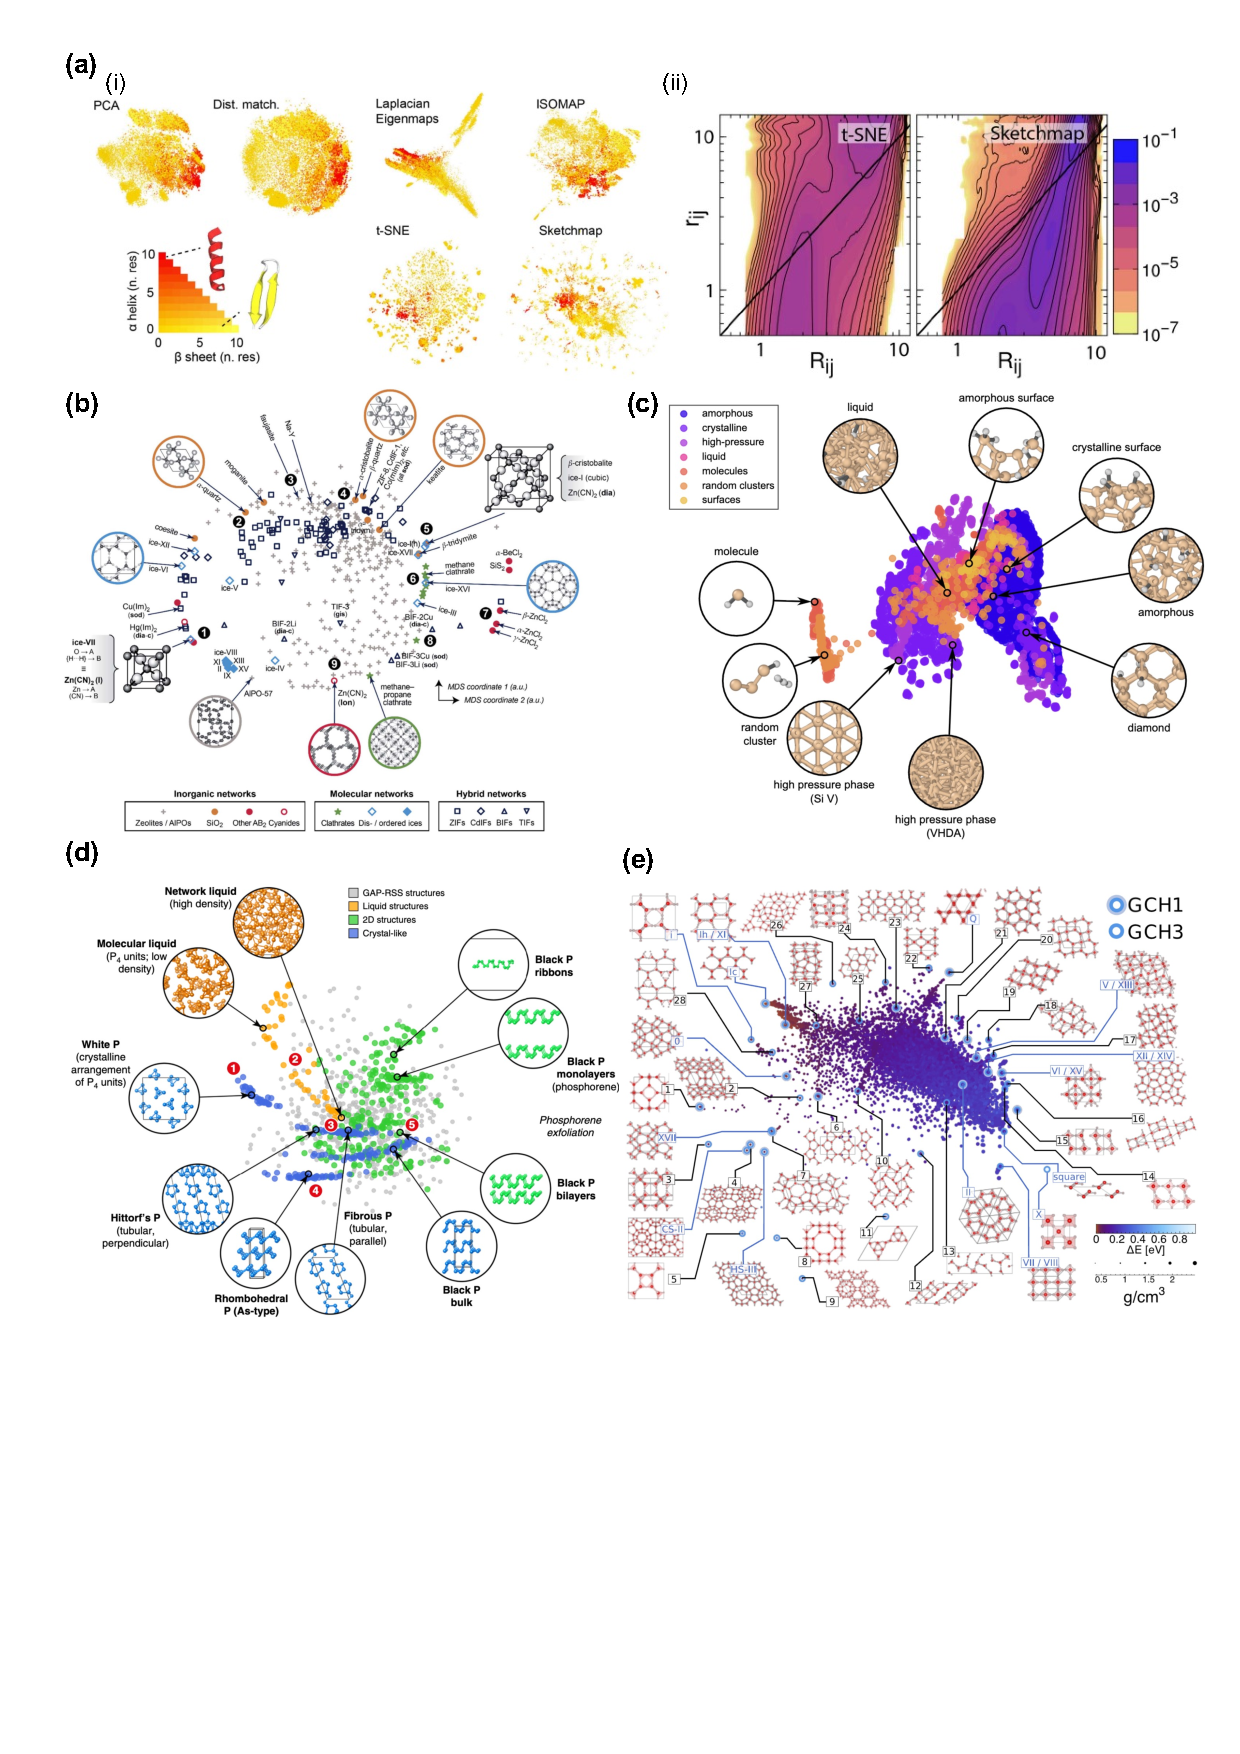
\includegraphics[width=0.96\textwidth]{MDS_maps_examples.pdf}
    \caption{Examples of MDS maps applied in analysing the atomistic molecular and materials modelling data, where the closer the two points are on the maps, the more similar are the corresponding atomistic structures of the two molecules/materials, and \textit{vice versa}. (a) (i) Comparison of different dimensionality reduction techniques in mapping the MD trajectories for immunoglobulin binding domain B1 of protein G, where each point is colour-coded based on the number of residues found in the $\alpha$-helix and $\beta$-sheet structures.\cite{tribello2019using} (ii) Histograms illustrating the joint probability distribution functions for the distances between configurations in the trajectory as measured in the orginal high-dimensional space ($R_{ij}$) and projected 2D manifold ($r_{ij}$) with the t-SNE\cite{van2008visualizing} and sketch-map\cite{ceriotti2011simplifying} methods. (b) A two-dimensional map comparing the inorganic and hybrid tetrahedral crystal packing frameworks, demonstrating how two groups of distinctively different material systems may adopt very similar crystal structures.\cite{nicholas2020understanding} (c) A two-dimensional map showing the diversity of structures in the Si-H dataset, encompassing molecular, liquid, crystalline, amorphous and high-pressure phases, that are used for training the cluster expansion potentials for the Si-H system.\cite{rosset2025atomic} (d) Similar technique applied to analyse the bulk and nanostructured phosphorus for forcefield training.\cite{deringer2020general} (e) Sketch map of 15,896 distinct PBE-optimised structures of ice.\cite{engel2018mapping} The mapping shows strong correlation between the positions of the projected point and the corresponding configurational energy (coloured coded) and the density (not shown here) of each ice polymorph. GCH is the shorthand for Generalised Convex Hull,\cite{anelli2018generalized} with corresponding structures circled on the sketch map.}
    \label{fig:MDS_maps_examples}
\end{figure}

\textbf{\textit{Multidimensional Scaling (MDS)}} Unlike the PCA-based techniques that are designed to capture the global trends across the entire dataset, MDS put more focus on preserving the local relationships among the data points. Another important difference between PCA and MDS lies in the fact that PCA leads to a definitive mapping from the original high-dimensional space to the low-dimensional space, while MDS, in its most general form that [\cref{eq:MDS_minimisation}] aims to minimise the target function (\emph{e.g.} through gradient-based minimisation), which is the difference between the distances among the data points in the original high-dimensional space ($R_{ij}$) and the distances among the corresponding projected points in the low-dimensional space ($r_{ij}$), cannot always guarantee that: (a) the global optimal or the same local optimal solution can be reached with different initial conditions, and (b) $R_{ij}=r_{ij}$ to be satisfied for \textit{all} pairs of data points.\cite{tribello2019using} 

As further shown in \cref{appendix:mds},  variants of MDS differ from each other in the designs of the target function, through placing different weights on preserving the local relationships among the data points in different \textit{length scales} based on some basic understanding on the problem at hand, such that the general consensus is that no single MDS approach is unequivocally better than the others.\cite{duan2013evaluation} For instance, \citet{tribello2019using} systematically compared the performance of different dimensionality reduction techniques for analysing the MD trajectories of biomolecules, and for the specific example of the immunoglobulin binding domain B1 of protein G [\cref{fig:MDS_maps_examples}(a)(i)], \emph{all the algorithms do a reasonable job of separating the configurations that are predominantly $\alpha$-helix-like from those that have a structure that is predominantly composed of $\beta$-sheets}. A useful diagnostic tool to evaluate the performance of different MDS approaches is to compare the joint probability distribution functions $p(R_{ij},r_{ij})$ to understand how the high-dimensional spatial relationships among the data points may have been distorted in the process of projecting the data onto the low-dimensional manifold [\cref{fig:MDS_maps_examples}(a)(ii)]. Similar finding was reached in our own work that analysed the crystal packing landscape of a flat acene-type molecule.\cite{yang2019interplay} As such, the aim of the subsequent discussion is to provide a few notable examples on how MDS has been applied to reveal the complex structural landscapes for some seemingly simple material systems.

Tetrahedron is one of the most common form of connectivities observed in the inorganic crystals, with \ce{SiO2} being probably the most well-known example, which is also adopted by many crystals of hybrid organic-inorganic materials. To show case this fundamentally important phenomenon, by allowing inorganic and hybrid crystals to be compared in the same footing, \citet{nicholas2020understanding} devised a coarse-graining and standardisation procedure, which led to a unified two-dimensional structural map [\cref{fig:MDS_maps_examples}(b)] that exemplifies the structural heterogeneity of the tetrahedral crystal packing frameworks across inorganic crystals, clathrate hydrates and zeolitic imidazolate frameworks (ZIFs). Such map may be used to facilitate the understanding on how similar properties among different material systems may arise from the similar local tetrahedral connectivities in their crystal structures.

\cref{fig:MDS_maps_examples}(c) shows the map of Si-H structures that are used for training the cluster expansion potentials for the Si-H system.\cite{rosset2025atomic} Unsurprisingly, the map shows the molecular and cluster Si-H structures are significantly distinct from the crystalline and amorphous structures, forming a separate `island' on the two-dimensional map. However, despite the fact that crystalline, amorphous, and liquid-like structures differ fundamentally in terms of long-range ordering, they can be projected to be close to each other due to the strong similarities in the local tetrahedral bonding environments around the Si atoms that are preserved in different phases of the Si-H system. Similarly approach has also been applied to analyse the bulk- and nano-structure landscape of phosphorus [\cref{fig:MDS_maps_examples}(d)],\cite{deringer2020general} which is another material system that is well-known to be highly polymorphic. 

Last but not least, \citet{engel2018mapping} charted the structural landscape of 15,896 distinct ice structures that are both known experimentally and generated from random structure searching. As shown in \cref{fig:MDS_maps_examples}(e), the sketch-map projection shows a strong correlation between the structure and energetic stabilities of ice polymorphs. A particular interesting application of this map is its combination with the concept of the Generalised Convex Hull (GCH),\cite{anelli2018generalized} which is a data-driven generalisation of the conventional concept of convex hull based on thermodynamic constraints, that in the structural descriptor space, identify the structurally most distinctive on the global scale yet energetically most stable amongst a set of structural neighbourhood.  

\begin{figure}[tbh]
    \centering
    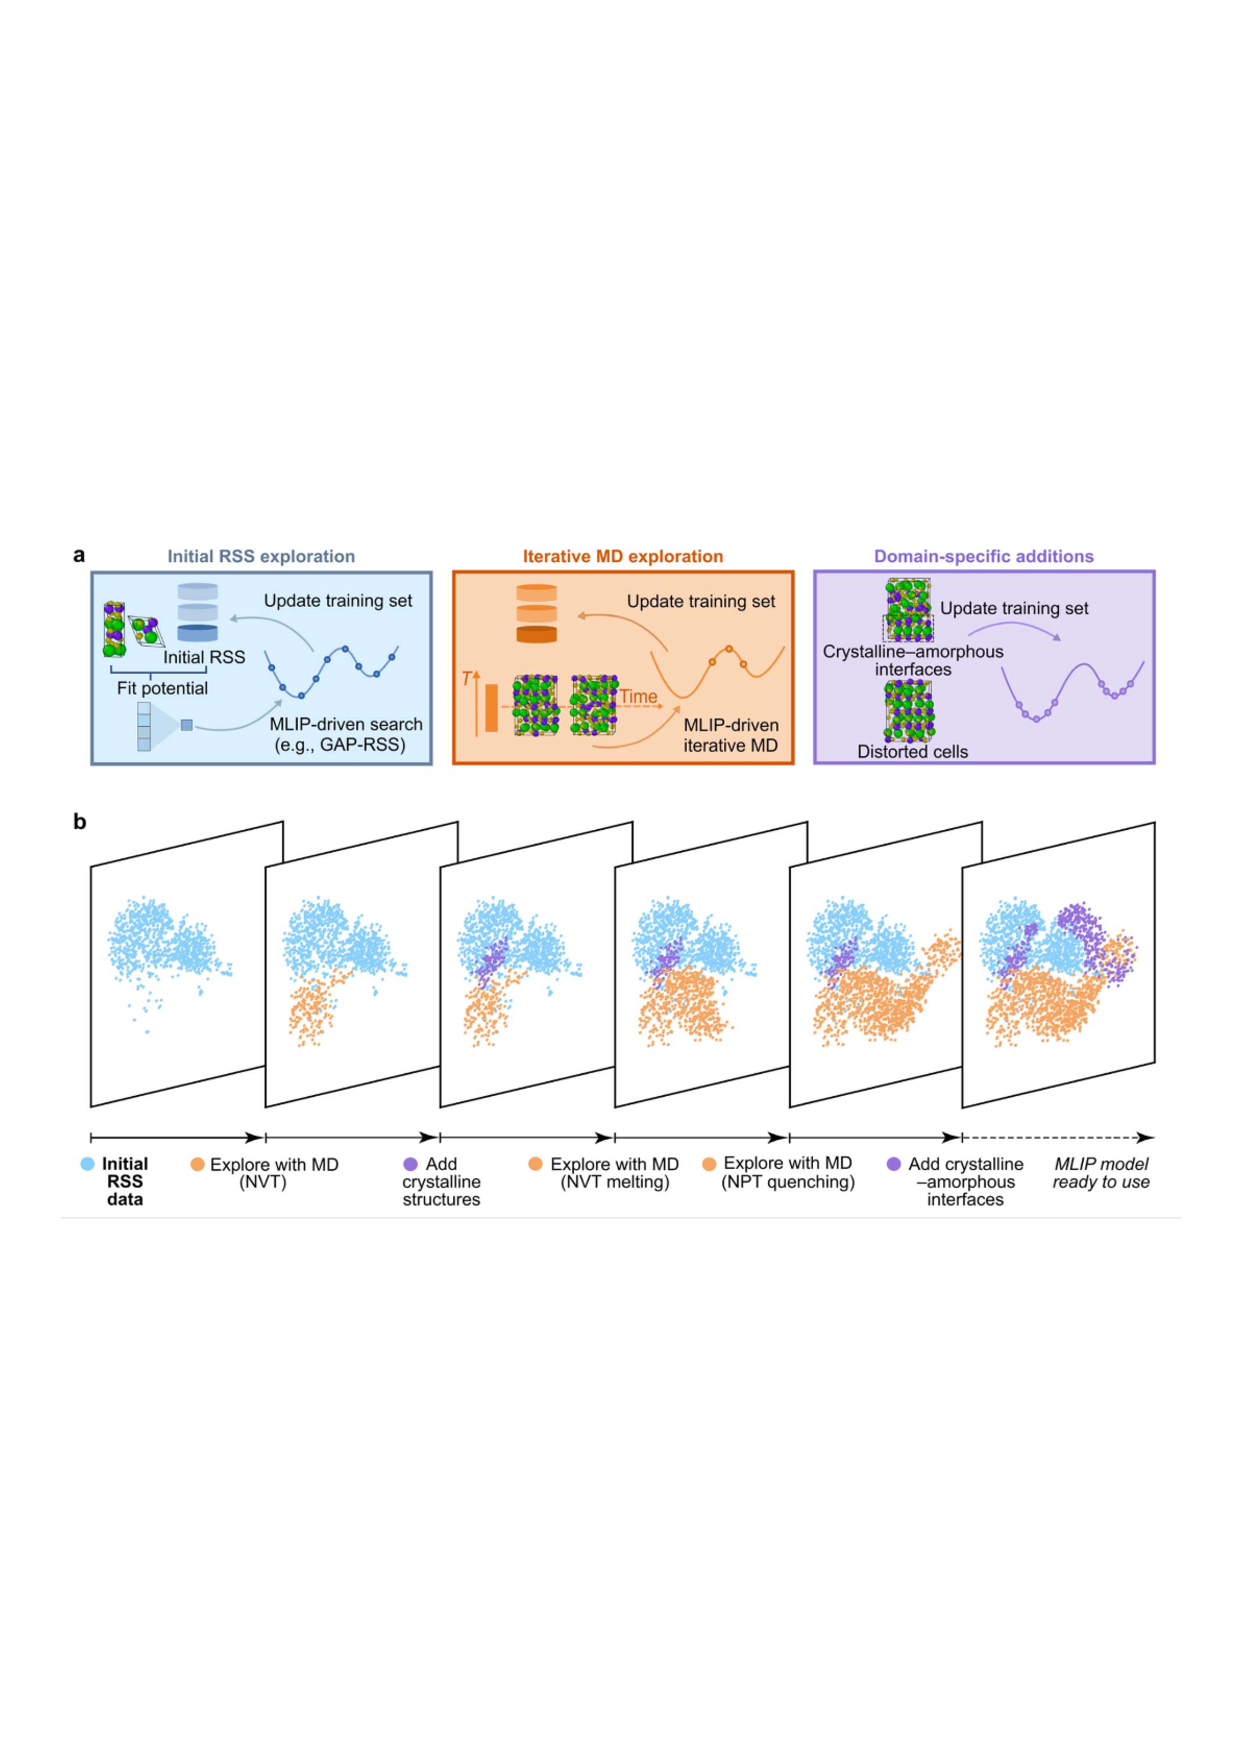
\includegraphics[width=0.85\textwidth]{MDS_sampling_model.pdf}
    \caption{Synergistics between supervised and unsupervised ML in the development of ML energy models for an exemplary system of crystalline and amorphous \ce{BaZrS3}.\cite{pacsca2025machine} The UMAP\cite{mcinnes2018umap} projections based on the SOAP\cite{bartok2013representing} structural descriptor are applied to demonstrate how training data generated with three different sampling approaches (panel a) are progressively incorporated into the training dataset (panel b) to enhance the coverage of the training dataset in the configurational space.}
    \label{fig:MDS_sampling_model}
\end{figure}

Finally, the coverage of the structural space plays a critical role in the development and validation of ML/AI-based energy models,\cite{fu2022forces,yang2026mace} particularly in sustaining long-time dynamic simulation of molecules and materials. As shown in \cref{fig:MDS_sampling_model}, unsupervised ML is a powerful tool for us to monitor the coverage of the training dataset in the configurational space, that is use to guide the training process of energy models, particularly to understand whether (a) the portion of the configurational space in which the trained model will be subsequently applied, and (b) likely regions in which the models need to be able to extrapolate to in the subsequent applications, have been sufficiently covered in the training dataset.

